% preamble and style file for M&R lecture slides
\documentclass[11.5pt,sans,english]{beamer}

\usetheme{EastLansing}
\usecolortheme{lily}

\usepackage[most]{tcolorbox}

\usepackage{verbatim}
%\usepackage{ulem}
%\usepackage{fontawesome}
%\usepackage{tikz}
%\usepackage{pifont}
%\usepackage{tabularx}
\usepackage{array,booktabs,xcolor,colortbl,multirow,rotating,amssymb}
%\usepackage{amsmath}
% \usepackage{vwcol}
% \usepackage[T1]{fontenc}

  
\newcommand\vect[1]{\underline{\mathbf{#1}}}
\newcommand\unitvect[1]{\hat{\boldsymbol{#1}}}
%\newcommand\hatdot[1] { \hat{ \dot{ \boldsymbol{#1} } } }

\newtcbox
{\keyc}{on line,arc=2pt, colback=yellow!30!white, colframe=yellow!30!black, before upper={\rule[-3pt]{0pt}{10pt} },boxrule=1pt,boxsep=0pt,left=6pt,right=6pt,top=2pt,bottom=2pt,}

\newtcbox
{\keyb}{on line,arc=1pt, colback=blue!30!white, colframe=blue!30!black, before upper={\rule[-3pt]{0pt}{10pt} },boxrule=1pt,boxsep=0pt,left=6pt,right=6pt,top=2pt,bottom=2pt,}

\newtcbox
{\keyl}{on line,arc=1pt, colback=pink!30!white, colframe=blue!30!black, before upper={\rule[-3pt]{0pt}{10pt} },boxrule=1pt,boxsep=0pt,left=6pt,right=6pt,top=2pt,bottom=2pt,}

\newtcbox
{\keyw}{on line,arc=1pt, colback=red!30!white, colframe=blue!30!black, before upper={\rule[-3pt]{0pt}{10pt} },boxrule=1pt,boxsep=0pt,left=6pt,right=6pt,top=2pt,bottom=2pt,}

\newtcbox
{\keya}{on line,arc=1pt, colback=purple!30!white, colframe=blue!30!black, before upper={\rule[-3pt]{0pt}{10pt} },boxrule=1pt,boxsep=0pt,left=6pt,right=6pt,top=2pt,bottom=2pt,}

\newtcbox[auto counter,number within=section]
{keyf}
{
enhanced,
on line,
  boxsep=0pt,
  left=6pt,right=6pt,top=2pt,bottom=2pt,
  arc=5pt,
  boxrule=1pt,
  rightrule=38pt,
colback=green!10!white, 
colframe=green!50!black, 
title=\thetcbcounter,
detach title,
overlay unbroken and first ={
    \node[%rotate=90,
          %minimum width=1cm,
          anchor=south,
          font=\sffamily\bfseries\tiny,
          %yshift=-10pt,
          yshift=-5pt,
          xshift=-20pt,
          white]
    at (frame.east) {\thetcbcounter};
  }
}


\usepackage{xcolor}

%\usepackage{hyperref}
%\hypersetup{
%  pdfauthor={Lily Asquith},
%  urlcolor=blue,
%  colorlinks=true,
%  linkcolor=blue,
%  bookmarks=true
%}

%---------------------------------------------%
%              LILY'S COLOURS           %
%---------------------------------------------%
\definecolor{Wash}{RGB}{204,204,204}
%\definecolor{Pinky}{RGB}{254,200,254}%violet
\definecolor{Pinky}{RGB}{219,	240,	253}%violet
\definecolor{Bluey}{RGB}{0,190,255}%deep sky blue
\definecolor{DarkGrey}{RGB}{28,66,137}%dar grey
\definecolor{SussexWhite}{RGB}{253,255,254}%dar grey
\definecolor{LightGray}{RGB}{184,184,255}
\definecolor{YesGreen}{RGB}{0,128,0}
\definecolor{NoRed}{RGB}{250,0,0}



\definecolor{myred}{RGB}{255,153,153}
\definecolor{myorange}{RGB}{255,204,153}
\definecolor{myyellow}{RGB}{255,255,153}
\definecolor{mygreen}{RGB}{153,255,153}
\definecolor{mycyan}{RGB}{153,255,255}
\definecolor{myblue}{RGB}{153,204,255}
\definecolor{myviolet}{RGB}{153,153,255}
\definecolor{mypurple}{RGB}{204,153,255}
\definecolor{mypink}{RGB}{255,204,255}
\definecolor{mycoral}{RGB}{255,153,204}

%-----------------------------------------------------%
%              LILY'S COLUMN TYPES          %
%-----------------------------------------------------%
\newcolumntype{a}{>{\raggedright\arraybackslash}l}	
\newcolumntype{q}{>{\raggedright\arraybackslash}m{8cm}} 

%--------------------------------------------%
%              LILY'S SYMBOLS          %
%--------------------------------------------%
\newcommand{\dfinger}{\large{\textcolor{black}{\ding{43}}}\scriptsize}
\newcommand{\dstar}{\large{\textcolor{black}{\ding{76}}}\scriptsize}
\newcommand{\dwrite}{\large{\textcolor{black}{\ding{45}}}\scriptsize}
\newcommand{\ddiamond}{\small{\textcolor{DarkGrey}{\ding{117}}}\scriptsize}
\newcommand{\ddiamondwhite}{\small{\textcolor{SussexWhite}{\ding{117}}}\scriptsize}
\newcommand{\experiment}{\small{\textcolor{magenta}{\faCogs }}\scriptsize}
\newcommand{\watchit}{\textcolor{blue}{ \faYoutube}}


\makeatletter
\newcommand\notsotiny{\@setfontsize\notsotiny{6.5}{7.5}}
\makeatother


% 
\title[ Intro to Quantum Physics]{Intro to Quantum Physics F3241}
%\subtitle{\textbf{Part 1: Preface}}
\author[Dr Lily Asquith (Lily)]{ Dr Lily Asquith (Lily)}
\date[27 Sep - 01 Oct 2021]{ 27 Sep - 01 Oct 2021 (Week 1)}
\logo{

\includegraphics[width=1.5cm]{../../utils/uslogo.jpg}
}


\begin{document}


\begin{frame}
\titlepage
\end{frame} 



 \begin{frame}{Recap : LMT dimensions}
To get a grip and do useful science, we should think about what it is important.\\
\begin{itemize}
\item Length [L]\\
\item Mass [M]\\
\item Time [T]\
\end{itemize}

The dimension of area is $L^2$. \\[1ex]
\begin{itemize}
\item[a] What is the dimension of volume?\\[1ex]
\item[b] What is the dimension of density (mass/volume)?\\[1ex]
\item[c] What is the dimension of acceleration?\\[1ex]
\item[d] What is the dimension of force?\\[1ex]
\item[e] What is the dimension of energy?\\[1ex]
\end{itemize}
\end{frame}
 




%-----------------------------------------------------
%     LECTURE 2
%-----------------------------------------------------

\subsection{Fundamental Constants \& Natural Units}
\begin{frame}{What is a fundamental constant?}

Things that change depending on where and when you measure them:\\[10ex]

Things that do not change depending on where and when you measure them:\\[10ex]


\end{frame}


\begin{frame}{The speed of light in a vacuum}

A lot of smart people in history thought that the light did not travel, or travelled at an infinite speed.\\[2ex]

How would you go about trying to measure the speed of light?\\[5ex]

Einstein proved that $c$ is constant in 1905 with his theory of Special Relativity.\\[2ex]

As measurements of $c$ became more sophisticated, the uncertainty on the definition of the metre became a problem\\[1ex]

%1983: $c = 2.99792458 \times 10^8$ metres per second (exact).\\

\end{frame}


\begin{frame}{The Atomic Clock}

In the 20th century, we started to realised that there were some things that were in fact more regular than clockwork, and more stable than lumps of metal\\[1ex]

The atom is like a mechanical clock!\\[16ex]


\end{frame}


\begin{frame}{Redefining the second  (1967)}
\small

The frequency of light emitted when a Caesium 133 atom undergoes a transition (a hyperfine ground state transition) was constant, enormous, and precisely measurable.\\[1ex]

The light associated with this transition had a measured frequency of 9.19263177 GHz:\\[6ex]

%\fbox{\begin{minipage}{0.4\textwidth}
\begin{center}
1s $ = \displaystyle  \frac{9.192631770 \times 10^{9}}{\Delta \nu_{Cs}} $\\[3ex]
 \end{center}
% \end{minipage}}

 \vspace{0.5cm}
 

Or equivalently:\\[1ex]

 $\Delta \nu_{Cs} = 9.192631770 \times 10^{9}$ Hz = $9.192631770 \times 10^{9}$ s$^{-1}$\\[1ex]
%1983: The metre is redefined as the distance travelled by light in a vacuum in 1/299,792,458 of a second.\\[1ex]

%Fundamental: measurements of $c$ are no longer meaningful. We have fixed its value to exactly that of the world best measurement, and redefined the units accordingly.\\[1ex]
\end{frame}



\begin{frame}{Redefining the metre (1983)}
\small

The speed of light in a vacuum must be constant according to special relativity. Using this, and the exact definition of a second, we can redefine the metre:\\[1ex]

%\fbox{\begin{minipage}{0.75\textwidth}
\begin{center}
1m $ = \displaystyle \left( \frac{9.192631770 \times 10^{9}}{\Delta \nu_{Cs}}\right)  \left( \frac{c}{2.99792458 \times 10^{8}}\right)  $\\[2ex]
 \end{center}
% \end{minipage}}
 \vspace{0.5cm}
 
Or equivalently, $c = 2.99792458 \times 10^{8}$ ms$^{-1}$\\[1ex]


Fundamental: measurements of $c$ are no longer meaningful. We have fixed its value to exactly that of the world best measurement, and redefined the units accordingly.\\[1ex]

\end{frame}


\begin{frame}{Redefining the kilogram (2019)}
\small
Planck's constant $h$ can be measured in all sorts of ways (as we shall see later), and is known very precisely from these measurements.\\[1ex]

We now use the fixed value of $h = 6.62607015\times10^{-34}$ (units?) to define the kilogram:\\[1ex]

%\fbox{\begin{minipage}{0.4\textwidth}
\begin{center}

1kg $ = \displaystyle  \left( \frac{9.192631770 \times 10^{9}}{\Delta \nu_{Cs}} \right)       \left( \frac{c}{2.99792458 \times 10^{8}}\right)        \left( \frac{h}{6.62607015\times10^{-34}}\right) $\\[2ex]
 \end{center}
% \end{minipage}}
 \vspace{0.5cm}

Note that we are \textbf{not} claiming to know the exact value of $h$ with no uncertainty, even though it kind of feels like we are.\\[1ex]

\end{frame}



\begin{frame}{Redefining the Ampere (and Coulomb)}
\small
The SI base unit Ampere is the unit of current, and the Coulomb is the unit of charge: 1  A = 1 Coulomb per  second\\[1ex]

We can measure the charge on an electron very precisely (as we shall see), and we know that all electrons have exactly the same charge\\[1ex]

The elementary charge $e = 1.602176634\times10^{-19}$ C\\[1ex]


\begin{center}
1 C $ = \displaystyle \frac{e}{1.602176634\times10^{-19}} $\\[2ex]
\end{center}

and so 

\begin{center}
1 A $ = \displaystyle \left( \frac{e}{1.602176634\times10^{-19}}\right)  \left( \frac{\Delta \nu_{Cs}}{9.192631770 \times 10^{9}}\right) $\\[2ex]
\end{center}


\end{frame}




\begin{frame}{The other three}
\small

We have used  $\nu_{Cs}$, $c$, $h$, and $e$ to define seconds, metres, kilograms, and Amperes.\\[2ex]

Three more fundamental constants $\rightarrow$ three more SI base units!\\[2ex]

$k_{B} = 1.380649\times10^{-23} $ Joules per Kelvin (base units?)\\[2ex]

$N_{A} = 6.02214076\times10^{23}$ per mole of stuff\\[2ex]

$K_{cd}$ = 683  candela - steradian -per kilogram -per metre squared -seconds cubed\\[2ex]



\end{frame}


\begin{frame}{Summary}
%\begin{columns}
%\begin{column}{0.4\textwidth}
%\small
%$\nu_{Cs}$: Frequency of  Cs-133.We use it to define the second.\\[1ex]
%
%$c$: the speed of light in a vacuum. Defines the metre.\\[1ex]
%
%$h$: Planck's constant. Defines the Kilogram.\\[1ex]
%
%$e$: The elementary charge. Defines the Ampere, Coulomb.
%\end{column}
%\begin{column}{0.6\textwidth}
\begin{center}
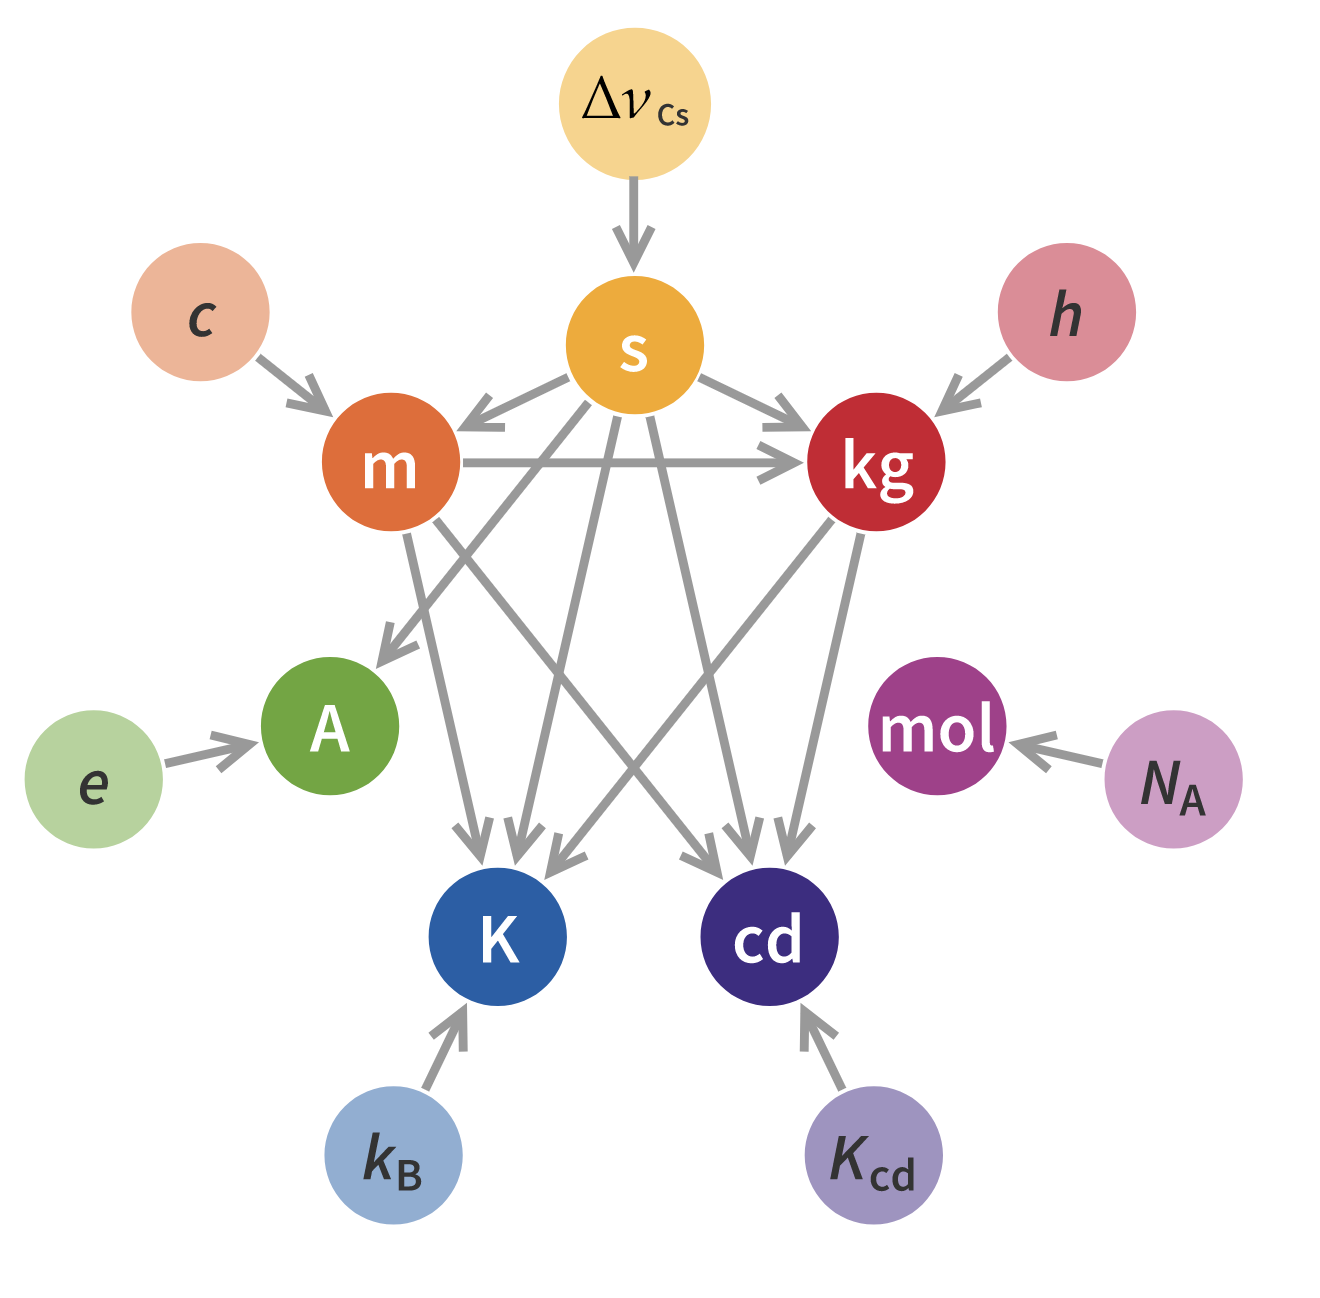
\includegraphics[scale=0.3]{SInew}
\end{center}
\tiny
By Emilio Pisanty - Own work, CC BY-SA 4.0
%\end{column}
%\end{columns}
\end{frame}

 \begin{frame}{Nobody's favourite constant (?) $N_A$}
 Avagadro's number $N_A$\\[1ex]
 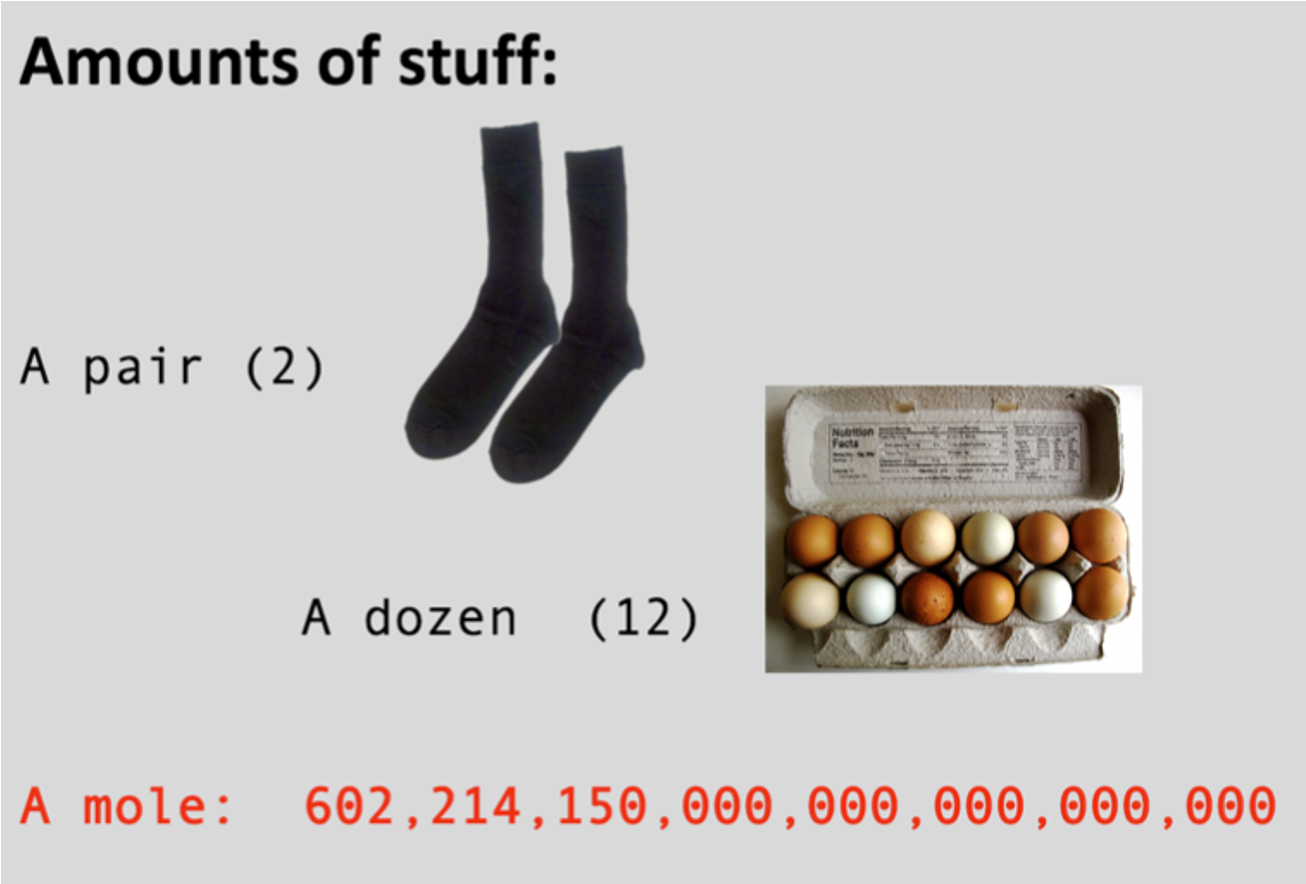
\includegraphics[scale=0.4]{avagad1}
 \end{frame}
 
  \begin{frame}{ Avagadro's number $N_A$ (1811)}
 $N_A = 6.02214076\times10^{23}$ mol$^{-1}$\\[1ex]
 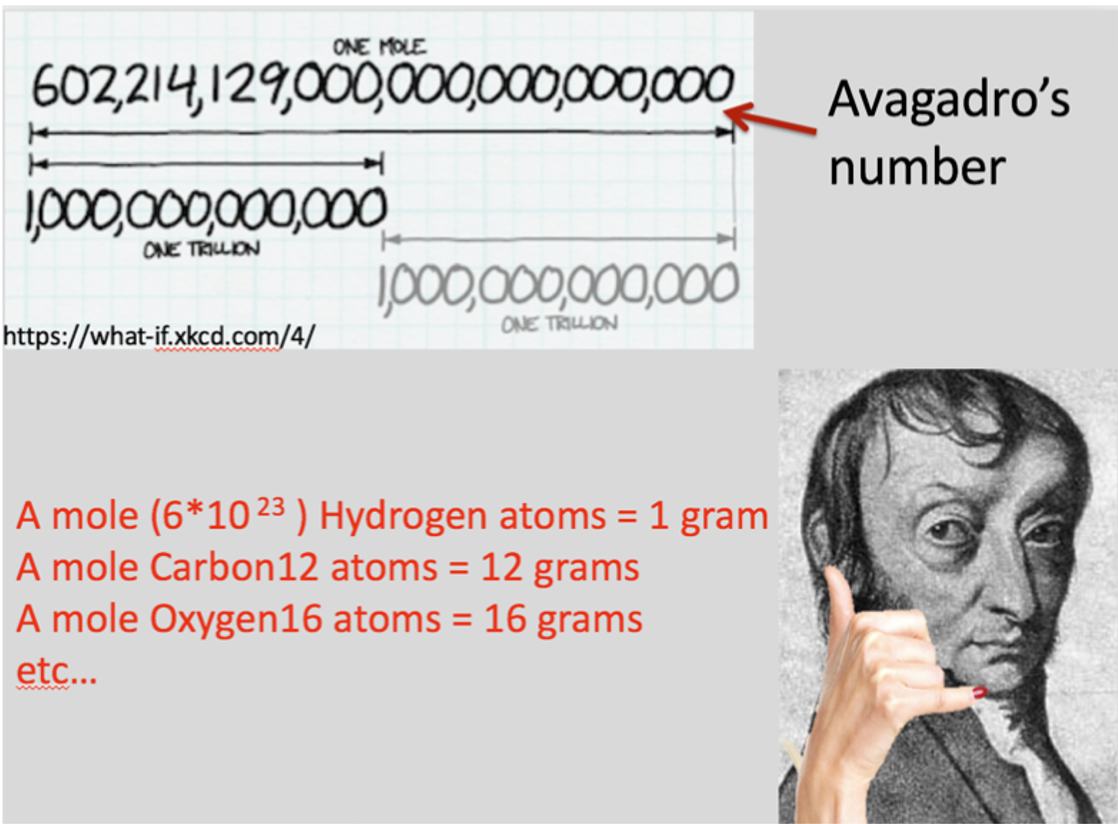
\includegraphics[scale=0.4]{avagad2}
 \end{frame}
 
 
 
\begin{frame}{Back to dimensions: L, T, M, I}
$\nu_{Cs}$ : \\[4ex]
 $c$ :\\[4ex]
 $h$ : \\[4ex] 
 $e$ : \\[4ex] 
 
\end{frame}

% \begin{frame}{ Three more useful physical constants}
% 
% We have used 7 fundamental physical constants to define 7 base units. It is useful to use three more constants:\\[1ex]
% 
% The mass of the electron $m_e = 9.109\times10^{-31} kg$ \\[2ex]
% The vacuum permittivity $\epsilon_0 = 8.8541878128(13)\times10^{-12}$ F m$^{-1}$ (Farads* per metre)\\[2ex]
% The reduced planck constant $\hbar = \frac{h}{2\pi}$\\[2ex]
% 
% Why? Because with these we can magically make our calculations MUCH simpler.\\[2ex]
% 
% 
% * The Farad is a measure of capacitance, which translates to kg$^{-1}$ m$^{-2}$ s$^{4}$ A$^{2}$\\[1ex]
% 
%
% \end{frame}


\begin{frame}{Natural Units}
\small

When dealing with complex formulae and tiny scales, it makes sense to adjust our system.\\[1ex]

$c = 2.99792458 \times 10^{8}$ ms$^{-1}$\\[1ex]

There exist some units in which I can write $c=1$. It still has the dimensions LT$^{-1}$, but it has the value 1.\\[1ex]

I could similarly do the same thing for other constants that appear regularly in the equations I have to solve.\\[1ex]

 \end{frame}
 
 
 
 
 
 \begin{frame}{ The electronVolt, eV}
 
 The electronVolt is a unit of energy that I use every single day.\\[2ex]
 
% $E = qV$ : the relationship between energy $E$, charge $q$, and potential difference $V$\\[2ex]
%An electron has elementary charge $e=1.6\times 10^{-19}$ C\\[2ex]
%So we can write $E_{e} = eV$ : the energy is an "electronVolt"\\[2ex]
 
 It is small: 1eV $=1.602176634\times10^{-19}$ J \\[2ex]
 
 A Joule is the energy required to accelerate a 1 kg mass at 1 ms$^{-2}$ through a distance of 1 m.\\[2ex]
 
 An electronVolt is the energy gained by an electron accelerated through a potential difference of 1 Volt in a vacuum.\\[2ex]
 
 %Notice: \\
 
 %1 C $ = \frac{e}{1.602176634\times10^{-19}} $\\[2ex]
 
 The eV is a better unit of energy for the kind of physics we are going to be doing.
 
 
 

 \end{frame}
 
 
\begin{frame}{ The electronVolt, eV}
 
1eV $=1.602176634\times10^{-19}$ kg m s$^{-2}$ : Energy in eV \\[2ex]

With this better unit for energy, and the understanding that there exist some units in which I can write $c=1$, we are all set.\\[2ex]

1eV =$1.782662\times10^{-36}$ kg ($\times c^{2}$) : Mass in eV \\[2ex]

1eV =$5.344286\times10^{-28}$ kg m s$^{-1}$ ($\times c$) : Momentum in eV\\[2ex]
 
\end{frame}


\begin{frame}{ Things in eV}

The mass of the electron:\\[2ex]
$m_e = 9.11\times10^{-31}$ kg $\rightarrow$ 510  keV\\[3ex]

Planck's constant multiplied by the speed of light:\\[2ex]
$hc = 1.99 \times10^{-25}$ Jm $\rightarrow $ 1.24 eV $\mu$m  \\[3ex]

So we get more manageable numbers, in addition to being able to seamlessly relate mass, energy, momentum, ...\\[3ex]

\end{frame}


\begin{frame}{ Fully Natural Units}
\small
In particle physics and similar fields, we use the \textbf{natural units}:\\

$c = 1$, $\hbar = 1$, $m_e = 1$, $\epsilon_0 = 1$\\[1ex]

Such that:\\[1ex]

1 s = $1.519 \times 10^{15}\; \hbar\;$ eV\\[1ex]
1 m = $5.068 \times 10^{6}\; c \hbar\;$ eV$^{-1}$\\[1ex]
1 kg = $5.610 \times 10^{35}\; c^{-2}\;$ eV\\[1ex]

Although this seems confusing now, you may gradually learn to love it over the next few years!
\end{frame}

 \begin{frame}{End of part 1.2}
End of part 1.2 : Constants\\[1ex]
Next lecture (Friday 4pm) will be on tips \& tricks to help you get the most out of this module.\\
\end{frame}
 
 
 

 
 
 
\end{document}